\section{Misura delle caratteristiche di IC SN74LS244 }
\subsection{Caratteristiche statiche}
Per tutta la sezione si è proceduto ad alimentare il circuito con una tensione di alimentazione $V_{cc} =$\SI{5.01 \pm 0.03}{\volt}.
\paragraph{Misure delle tensioni d'operazione}
Per effettuare la misura delle tensioni operative di una porta NOT si 
è montato il circito in \figurename{ \ref{f:c1}}
\begin{figure}[h]
	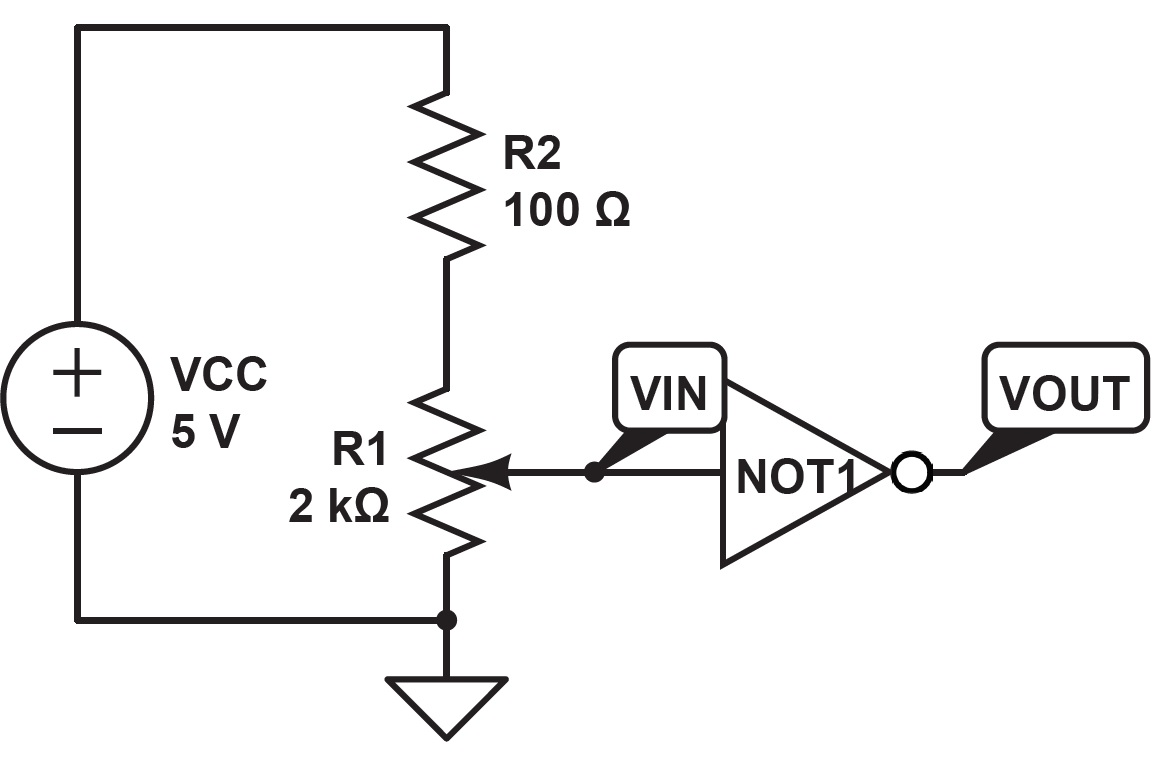
\includegraphics[scale=1.0]{../Figs-Tabs/immagine1.png}
	\caption{Rappresentazione del primo circuito impiegato.}
	\label{f:c1}
\end{figure} ,
dopodiché si è andati a  campionare la tensione in uscita, $V_{out}$, in funzione della tensione di ingresso , $V_{in}$.

Il circuito in  \figurename{ \ref{f:c1}} permette la variazione di  $V_{in}$ variando la resistenza del trimmer $R_{1}$;infatti esso  rappresenta un partitore di tensione.

Per la costruzione circuitale sono state impiegate: un trimmer $R_{1}$ di valore massimale $R_{1}^{max}=$\SI{94.0 \pm 0.8 }{\kilo \ohm} ed na resistenza $R_{2}=$\SI{100.8 \pm 0.9 }{ \ohm}.

Si riportano i dati campionati in \tablename{ \ref{t:1}}
\begin{table}[hb]
	\centering
	\begin{tabular}{|s|s|}
		\toprule
		V_{in} [\si{\volt}] & 	V_{out} [\si{\volt}]\\
		\midrule
		0	\pm 1e-3 & 4.38 \pm 0.02\\
		0.265 \pm 0.002 & 4.23 \pm 0.02\\
		0.584 \pm 0.003 & 4.02 \pm 0.02\\
		0.780 \pm 0.004 & 3.87 \pm 0.02\\
		0.881 \pm 0.005 & 3.78 \pm 0.02\\
		0.945 \pm 0.005 & 3.44 \pm 0.02\\
		1.003 \pm 0.005 & 2.95 \pm 0.02\\
		1.065 \pm 0.006 & 2.01 \pm 0.01\\
		1.103 \pm 0.008 & 0.1773 \pm 0.009\\
		1.238 \pm 0.009 & 0.1728 \pm 0.009\\
		1.56 \pm 0.01 & 0.1728 \pm 0.009\\
		1.775 \pm 0.02 & 0.1728 \pm 0.009\\
		1.991 \pm 0.02 & 0.1727 \pm 0.009\\
		2.52 \pm 0.02 & 0.1727 \pm 0.009\\
		3.02 \pm 0.02 & 0.1726 \pm 0.009\\
		3.48 \pm 0.02 & 0.1726 \pm 0.009\\
		3.93 \pm 0.02 & 0.1726 \pm 0.009\\
		5.00 \pm 0.03 & 0.1726 \pm 0.009\\
		\bottomrule
	\end{tabular}
	\caption{Si riportano i valori corrispondenti alle nostre acquisizioni.I dati campionati sono stati ottenti col multimetro digitale.
		Si è associato alle misure l'incertezza di un  digit sulla prima cifra che risultasse instabile sommata in quadratra con eventali errori di calibrazione del mltimetro.}
	\label{t:1}
\end{table}
.
Effettando un grafico  ( \figurename{ \ref{f:i1}} )
dei dati in  \tablename{ \ref{t:1}}, ( a cui sono stati scorporati gli errori di calibrazione del multimetro essendo uniformi per le scale impiegate) si osservano i valori di :\\
$V_{I,H}$, tensione in ingresso associata all'uscita HIGH;\\
$V_{I,L}$, tensione in ingresso associata all'uscita LOW;\\
$V_{O,H}$, tensione in uscita  associata all'uscita HIGH;\\
$V_{O,L}$, tensione in uscita associata all'uscita LOW.\\

Essendo tali valori da intendersi come intervalli di tensione si sono osservati i loro valori superiori ed inferiori ottenendo :
\begin{center}
	$V_{I,H}^{max}\sim$\SI{0}{\volt} \\
	$V_{I,H}^{min}=$\SI{1.003 \pm 0.005}{\volt}\\
	$V_{I,L}^{max}=$\SI{5.00 \pm 0.03}{\volt}\\
	$V_{I,L}^{min}=$\SI{1.108 \pm 0.008}{\volt}\\
	
	$V_{O,H}^{min}=$\SI{2.95 \pm 0.02}{\volt}\\
	$V_{O,H}^{max}=$\SI{4.38 \pm 0.02}{\volt}\\
	$V_{O,L}^{min}=$\SI{0.1726 \pm 0.0009}{\volt}\\
	$V_{O,L}^{max}=$\SI{0.1773 \pm 0.0009}{\volt}	\\
\end{center}

Tali stime risultano essere meno restrittive dei  valori
forniti dal costruttore nel datasheet:
\begin{center}
	
	$V_{O,H}^{min,atteso}=$\SI{2.4}{\volt}\\
	$V_{O,L}^{max,atteso}=$\SI{0.4}{\volt}\\
	$V_{I,H}^{min,atteso}=$\SI{2}{\volt}\\
	$V_{I,L}^{max,atteso}=$\SI{0.8}{\volt}.\\
\end{center}
Si imputa che questa lieve discrepanza 
con i valori attesi, sia dovuta al fatto che essi siano misurati nelle peggiori condizioni di operatività possibili della porta NOT.

Durante la fase di presa dati è stato osservato inoltre che nella regine di tensione compresa tra 	$V_{I,L}^{max}$ ed $V_{I,H}^{min}$ il segnale in uscita, risultasse variare tra lo stato HIGH e LOW,senza un apparente continuita.
Questo effetto risulta compatibile col fatto che il NOT non sia forzato ne nella regione $V_{O,H}$ ne in $V_{O,L}$; pertanto  l'uscita risulta indeterminata tra il regime di uscita high e low.
\begin{center}
	\begin{figure}[h]
		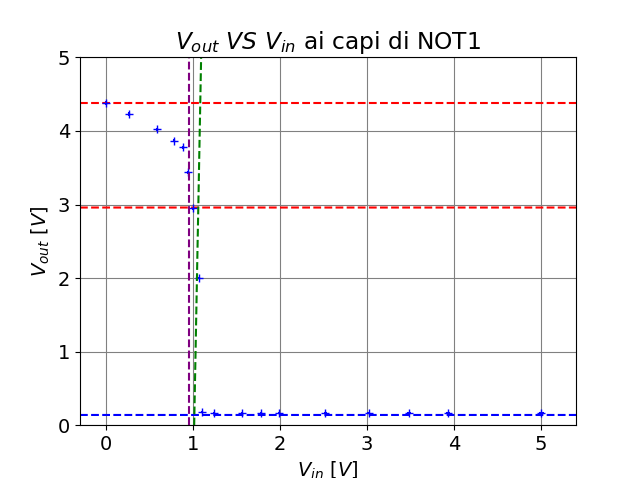
\includegraphics[scale=0.50]{../Figs-Tabs/in-ot2.png}
		\caption{Rappresentazione dei dati in \tablename{ \ref{t:1}}.}
		\label{f:i1}
	\end{figure}
\end{center}


\paragraph{Misura delle correnti e stima del fanout}
	Si è procedto d'apprima alla misura della corrente di ingresso.
	Per fare ciò si è modificato il circito in \fig{i1} inserendo in serie tra il trimmer e la porta logica il multimetro in configrazione amperometro.

	Avendo assunto che il fabbisogno di corrente della porta logica dipenda 	dallo stato di funzionamento (ingresso alto o ingresso basso)
	si è andati a imporre un segnale di $V_{IH} =$ \SI{4.73\pm 0.01}{\volt} osservando una corrente $I_{IH} \lessapprox$ \SI{0.5e-10}{\micro \ampere} (si è scelto di usare il multimetro digitale come voltmetro per la misura di $V_I$ ed il multimetro analogico come amperometro per la misura di $I_I$, dal momento che quest'ultimo è in grado di misurare correnti molto più basse, ma $I_{IH}$ resta troppo piccola per poter essere misurata, con uno spostamento dallo zero inferiore alla mezza tacca con il fondoscala più basso disponibile);
	analogamente si è posto per la misura di  $I_{IL}$ una tensione in ingresso $V_{IL} =$ \SI{0.1525(1)}{\volt} rilevando una corrente di \SI{-25}{\micro \ampere}. Si sono poste positive le correnti entranti nella porta logica e consegentemente negative quelle uscenti.

	Al variare della tensione in ingresso $V_{I}$ rimanendo entro il rispettivo range di funzionamento per ingresso alto o basso le correnti rilevate non cambiano significativamente; tali valori sono ampiamente entro i valori massimi riportati dal datasheet.

	Si è proceduto dunque alla misura delle correnti in uscita $I_{OL}$ ed $I_{OH}$, ovvero rispettivamente quelle rilevate in uscita alla porta logica per lo stato di output basso ed output alto; per fare ciò si è montato il circuito in \fig{c2}.

	\begin{figure}[h]
		\centering
		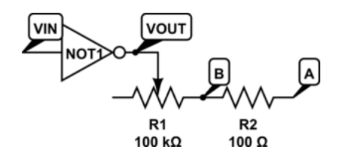
\includegraphics[scale=0.75]{cir2.png}
		\caption{Circuito impiegato per la misurazione di $I_{OL}$ e $I_{OH}$. }
		\label{f:c2}
	\end{figure}

	Dove i valori misurati dei componenti utilizzati sono:\\
	$R_{2}= $\SI{100.8 \pm 0.1}{\ohm}\\
	$R_{1,max}=$ \SI{94.0 \pm 0.1 }{ \kilo \ohm}\\

	Per ottenere le correnti in uscita si è misurata la caduta di potenziale  $V_2$ ai capi di $R_{2}$ con il multimetro digitale; per effettuare le misure di $I_{OL}$ si sono posti $V_{in}$ e $V_A$ alla tensione di alimentazione $V_{CC}=$\SI{5.01 \pm 0.1}{\volt}, mentre per $I_{OH}$ si sono poste le tensioni precedenti a terra. La convenzione sui segni è la
	stessa della misura della corrente in ingresso: le correnti entranti
	nel dispositivo sono positive, quelle uscenti negative.

	Si osserva in entrambi i casi come al variare della resistenza del
	potenziometro la corrente vari dapprima lentamente per poi aumentare
	bruscamente (supponiamo al raggiungimento dei limiti del dispositivo) in
	corrispondenza del discostarsi della tensione in uscita dall'intervallo di
	corretto funzionamento; le misure raccolte sono riportate in \tab{iout}.

	\begin{table}[h]
		\centering
		\begin{tabular}{SS cc SS}
			\toprule
			\multicolumn{2}{c}{Uscita bassa} &&& \multicolumn{2}{c}{Uscita alta} \\
			\cmidrule{1-2} \cmidrule{5-6}
			{$I_{OL}$ [\si{\mA}]}	& {$V_{out}$ [\si{\V}]}	&&& {$I_{OH}$ [\si{\mA}]}	& {$V_{out}$ [\si{\V}]} \\
			\midrule
			0.0506 (12)	&	0.1758 (10)	&&&	-0.0437 (12)	&	4.12 (3)	\\
			0.2679 (23)	&	0.1868 (10)	&&&	-0.0873 (14)	&	3.93 (3)	\\
			0.328 (3)	&	0.1904 (11)	&&&	-0.1270 (16)	&	3.77 (3)	\\
			1.553 (9)	&	0.2330 (22)	&&&	-0.1637 (18)	&	3.63 (3)	\\
			2.897 (24)	&	0.2660 (23)	&&&	-0.2937 (25)	&	3.53 (3)	\\
			5.21 (4)	&	0.320 (3)	&&&	-3.77 (3)	&	3.28 (3)	\\
			24.01 (22)	&	1.891 (10)	&&&	-13.31 (8)	&	2.300 (21)	\\
			27.88 (24)	&	1.988 (11)	&&&	-16.91 (9)	&	1.860 (10)	\\
			\bottomrule
		\end{tabular}
		\caption{Andamento dell'uscita della porta not al variare della corrente erogata.}
	\label{t:iout}
	\end{table}

	Si osserva che i valori risltano speriori a qelli forniti dal datasheet;
	tale discrepanza è imptabile alla differenza di condizioni operative in ci sono effettate le misre riportate rispetto a qelle del datasheet;
	n lteriore rogione per tale discrepanza pò essere dovta alla difficoltà nell'individare di massimo della tensione di soglia a casa della sensibilità del trimmer.

	La regione di discontinità presentata nell'andamento di $V_{R_{3}}$
	pò essere dovto al fatta che variando $R_{4}$ la richiesta di corrente fornita alla porta logica spera il valore massimo da essa erogabile;pertanto la tensione $V_{ot}$ amenta per ridrre il fabbisogno di corrente.
	Pertanto le parta NOT ed in particolare i transistor vengano spostati dalla regione di operatività lineare sino ad scire da  essa.

	Da i valori ottenti e dall'\eqref{eq:fan-o} si ottiene $$N=$$; tale valore rislta maggiore di qello fornito nel datasheet; tale effetto si è imptata come fatto per le correnti al fatto che i valori forniti dal costrttore sono valori misrati in condizioni estremali della regione di operatività.

\section{Montaggio arduino}
Per la verifica delle caratteristiche dinamiche dell'IC SN74LS244 si è montato un circito impulsatore, basato su di un microcontrollore arduino; successivamente impiegato come generatore di onde. 

Si riporta lo schema circitale in \figurename{ \ref{f:impulsatore}}. 

\begin{figure}[htb]
	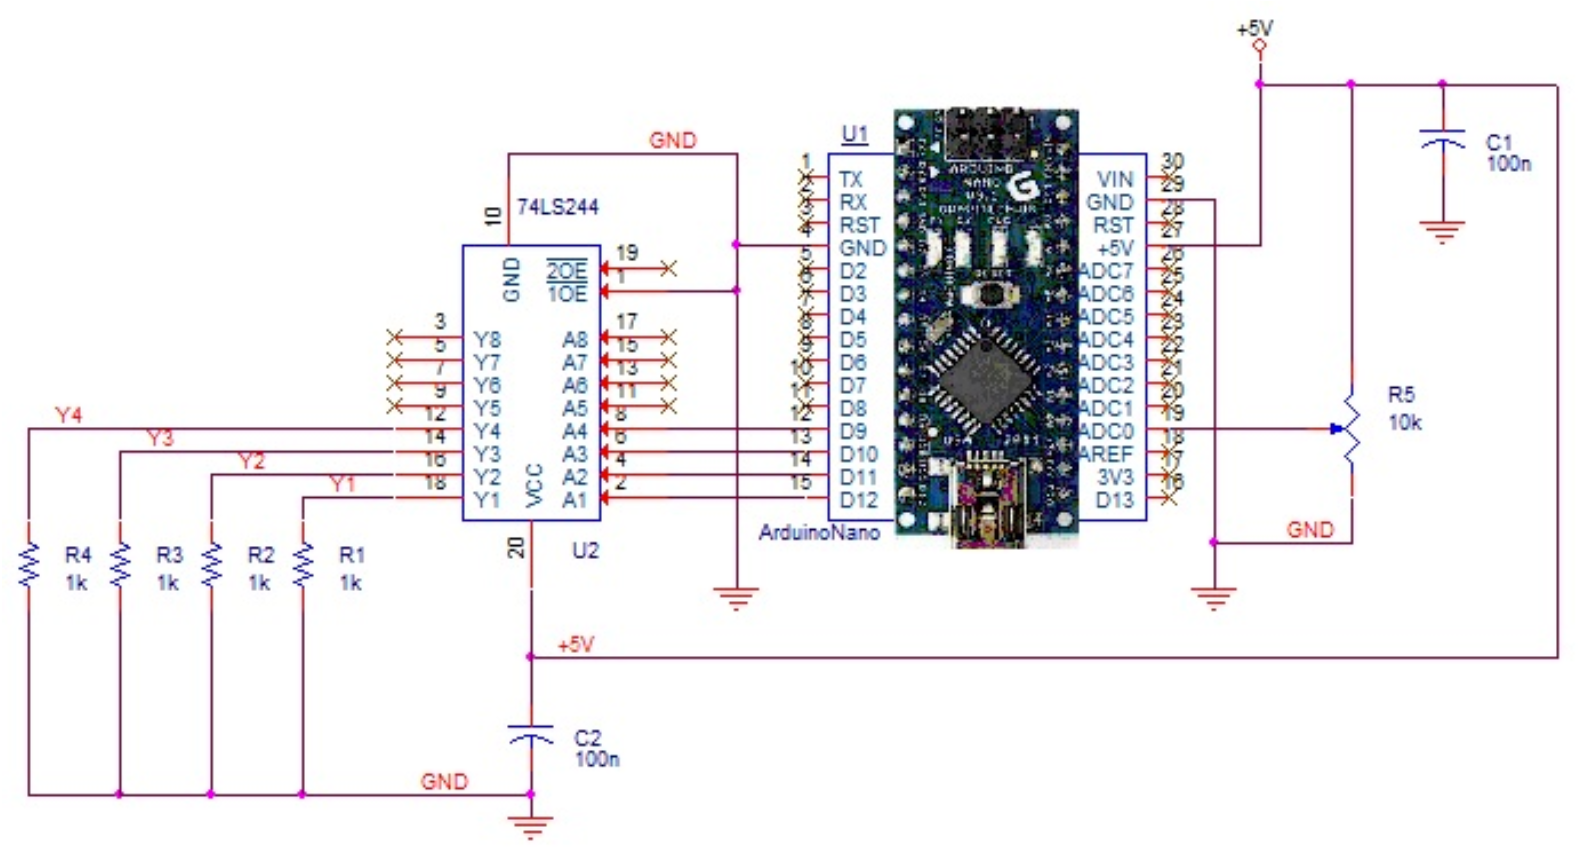
\includegraphics[scale=0.50]{../Figs-Tabs/imp.png}
	\caption{Rappresentazione del circuito impulsatore montato.}
	\label{f:impulsatore}
\end{figure}
Per il montaggio sono state impiegate le  segenti componenti circitali:
\begin{center}
	\bigskip
	$R_{1}=$\SI{984 \pm 8}{\ohm} $R_{2}=$\SI{984 \pm 8}{\ohm} $R_{3}=$\SI{982 \pm 8}{\ohm} \\
	$R_{4}=$\SI{983 \pm 8}{\ohm} n trimmer di $R_{5}^{max}=$\SI{10.2 \pm 0.8}{\kilo \ohm} \\
	dei condensatori	$C_{1}=$\SI{114 \pm 6 e-9}{\farad} $C_{2}=$\SI{114  \pm 6 e-9}{\farad}
	
\end{center}
Si segnala inoltre 
che da questa sezione si è impiegata una tensione di alimentazione $V_{cc}=$\SI{4.87 \pm 0.03}{\volt}; tale accorgimento è stato impiegato per evitare di danneggiare il microcontrollore arduino, sensibile per tensioni superiori a \SI{5}{\volt}.

Il circuito montato tra i terminali Y1 e Y2 dovrebbe generare delle onde quadre sfasate di $\pi/2$ , di frequenza regolabile attraverso il valore di $R_{5}$, e  compresa tra 50 Hz e 50KHz.

Si è andati pertanto a verificarne il corretto montaggio attraverso la verifica di queste proprietà.
Attraverso l'oscilloscopio si sono visalizzati su ch1 la tensione rilevata su Y1 e su  ch2 la tensione letta su Y2. Si riporta una tipica acquisizione in 
\figurename{ \ref{f:oscil} }.
\begin{figure}[htb]
	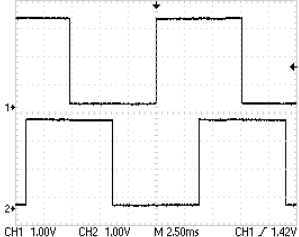
\includegraphics[scale=0.50]{../Figs-Tabs/ondaquadra_esempio.png}
	\caption{Tipica acqisizione delle tensioni lette si terminali Y1 (ch1) e Y2 (ch2) del circuito impulsatore.}
	\label{f:oscil}
\end{figure}

Come è possibile osservare dall'acquisizione la forma d'onda presentata dalle due tracce può essere trattata quale un onda quadra; si osserva inoltre che al variare del valore della resistenza $R_{5}$ la frequenza delle tracce assume valori compresi nell'intervallo $f\in [\sim 10 \text{Hz;} \sim 50 \text{KHz}]$.

Come ultima verifica dell'operatività del circuito montato si e proceduto a misurare lo sfasamento tra le due tracce.
Per fare ciò si è andati a misurare il $\Delta t$ tra i fronti di salita delle dei due canali, ottenendo $\Delta t=$\SI{248 \pm 2}{\mu \sec}\footnote{misura effettuata con i cursori dell'oscilloscopio in dotazione.} a fronte di una frequenza
$f=$\SI{1.007 \pm 0.001}{\kilo \hertz}\footnote{la misura di frequenza è stata effettuata con la funzione di lettura automatica dell'oscilloscopio; a cui abbiamo abbiamo associato l'incertezza di un digit sulla cifra precedente alla prima che risultasse instabile. } .
Essendo valida la relazione \begin{equation}
\Delta \phi = 2 \pi \cdot f \cdot \Delta t
\end{equation}\label{eq:sfas}
si ottiene $\Delta \phi=$\SI{1.57 \pm 0.01 }{\radian} ,compatibile con $\phi/2$.

Visto l'accordo tra le richieste operative ed il funzionamento del circuito impulsatore montato 
si è assunto  come  corretta la realizzazione dello stesso.

\section{Caratteristiche dinamiche}
	SI vogliono studiare le caratteristiche dinamiche della porta NOT, per farlo si è inviata all'ingresso della stessa un' onda quadra (generata dalla scheda Arduino, configurata come al punto precedente) di frequenza  $f\sim$\SI{1}{\kilo \hertz} e tensione picco picco $V=$\SI{3.40 \pm 0.20}{\volt}.

	\subsection{Tempi di propagazione}
	Si è misurato il tempo $\Delta t_{PHL}$ che intercorre tra il centro del fronte di discesa all'ingresso e il centro del fronte di salita sull'uscita. Si è poi ripetuta la misura per $\Delta t_{PLH}$: il passaggio dal fronte di discesa (input) al fronte di salita (output).
	Per determinare il centro dei fronti di salita/discesa si è preso il punto in cui i segnali assumevano la metà del loro valore HIGH, ignorando quindi la presenza di overshoot e undershoot, visibili in \figurename{ \ref{f:ripple}}.

	\begin{figure}[H]
		\centering
		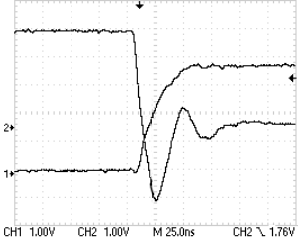
\includegraphics[scale=1]{undershoot_lh.png}
		\caption{Undershoot del segnale in uscita}
		\label{f:ripple}
	\end{figure}
	\noindent Per la misura si è scelta la scala che ottimizzava la risoluzione, ottenendo:
	$$\Delta t_{PHL}=\SI{9.6(6)}{\nano \second} \qquad \text{e} \qquad \Delta t_{PLH}=\SI{14.8(6)}{\nano \second}$$
	tali valori risultano in accordo con i valori attesi dal datasheet, che sostiene che entrambi i parametri debbano essere minori di \SI{15}{\nano \second}.
	
\subsection{Tempi di salita e discesa}
Si sono misurati i tempi di salita $\Delta t^{\uparrow}$ e discesa $\Delta t^{\downarrow}$ del segnale tra il $10 \% $ e il $90 \% $ del valore HIGH, sia in ingresso che in uscita. Si è ottenuto:
$$ \Delta t_{in}^{\uparrow}=\SI{12.2(6)}{\nano \second} \qquad \Delta t_{in}^{\downarrow}=\SI{6.4(6)}{\nano \second} $$
$$ \Delta t_{out}^{\uparrow}=\SI{16.4(6)}{\nano \second} \qquad \Delta t_{out}^{\downarrow}=\SI{48.8(1)}{\nano \second}.$$
